\documentclass[tikz,border=12pt]{standalone}
\usepackage[T1]{fontenc}
\usepackage{lmodern}
\usetikzlibrary{arrows.meta,calc,positioning,shapes.geometric}

\definecolor{llmblue}{HTML}{1565C0}
\definecolor{replorange}{HTML}{E65100}
\definecolor{finalgreen}{HTML}{2E7D32}
\definecolor{humanviolet}{HTML}{6A1B9A}
\definecolor{textgray}{HTML}{455A64}
\definecolor{softgray}{HTML}{ECEFF1}

\begin{document}
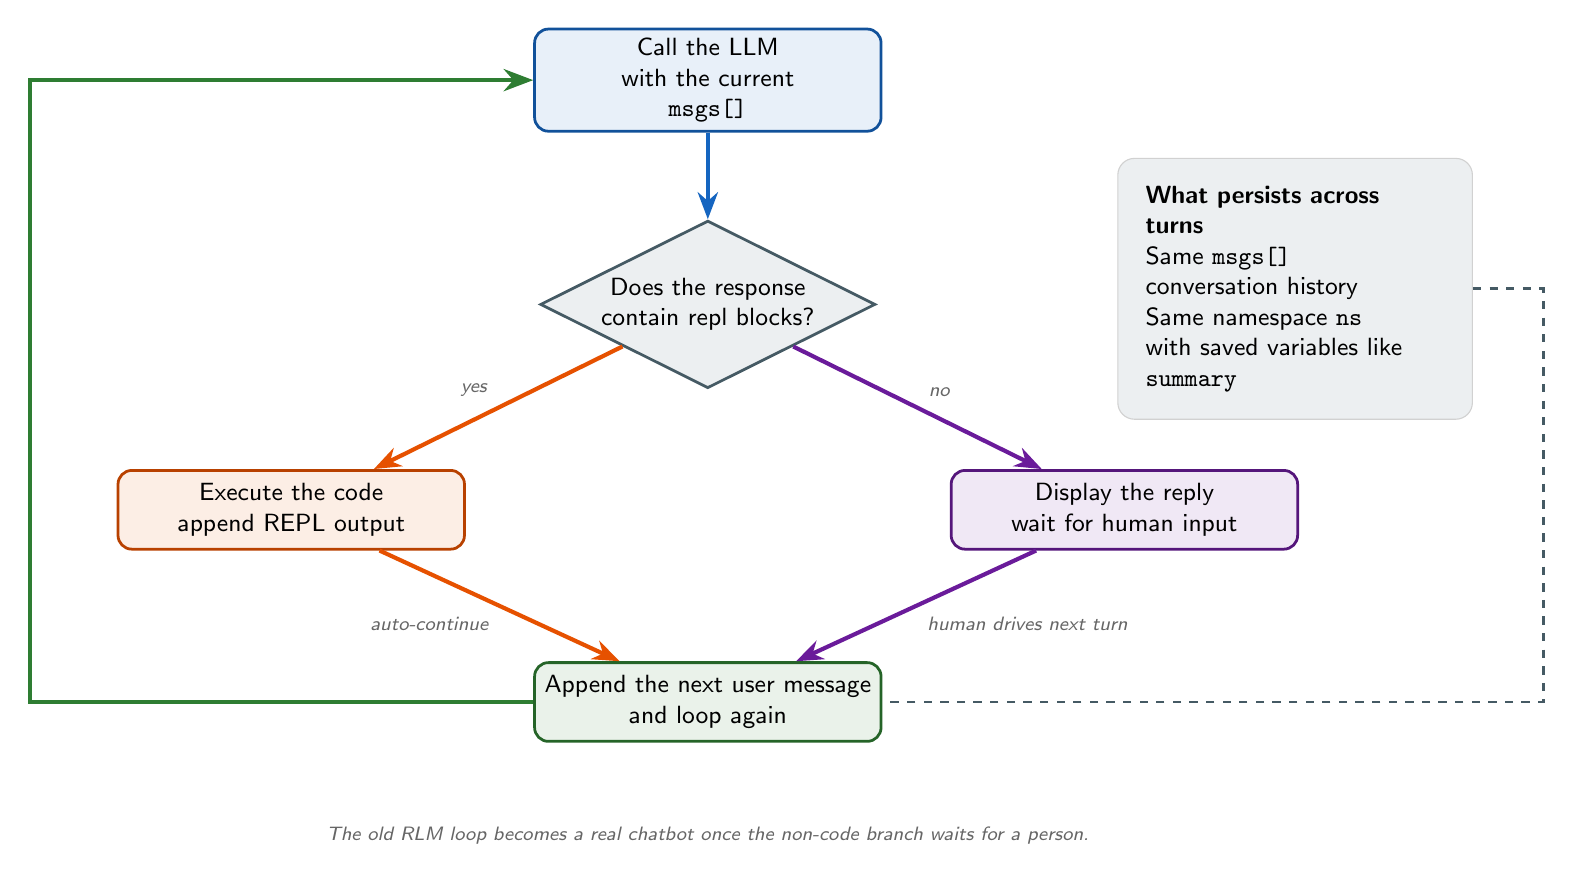
\begin{tikzpicture}[
		>=Stealth,
		font=\sffamily\small,
		block/.style={draw=#1!80!black, fill=#1!10, rounded corners=5pt,
				minimum width=4.4cm, minimum height=1cm, align=center,
				line width=1pt},
		decision/.style={diamond, draw=textgray, fill=softgray, aspect=2,
				align=center, inner sep=1pt, minimum width=3.2cm, minimum height=1.5cm,
				line width=1pt},
		note/.style={font=\sffamily\scriptsize\itshape, text=black!60, align=center},
		sidebox/.style={draw=black!18, fill=softgray, rounded corners=6pt,
				inner sep=10pt, align=left, text width=3.8cm},
	]

	\node[block=llmblue] (llm) at (0, 2.8)
	{Call the LLM\\with the current\\\texttt{msgs[]}};

	\node[decision, below=1.1cm of llm] (decision)
	{Does the response\\contain repl blocks?};

	\node[block=replorange, below left=1.55cm and 2.0cm of decision] (exec)
	{Execute the code\\append REPL output};

	\node[block=humanviolet, below right=1.55cm and 2.0cm of decision] (display)
	{Display the reply\\wait for human input};

	\node[block=finalgreen, below=3.45cm of decision] (append)
	{Append the next user message\\and loop again};

	\node[sidebox, anchor=west] (persist) at (5.2, 0.15) {
		\parbox{3.4cm}{\raggedright
			\textbf{What persists across turns}\\
			Same \texttt{msgs[]} conversation history\\
			Same namespace \texttt{ns} with saved variables like \texttt{summary}}
	};

	\draw[->, line width=1.5pt, llmblue] (llm) -- (decision);
	\draw[->, line width=1.5pt, replorange] (decision) -- (exec)
	node[midway, above left, note] {yes};
	\draw[->, line width=1.5pt, humanviolet] (decision) -- (display)
	node[midway, above right, note] {no};
	\draw[->, line width=1.5pt, replorange] (exec) -- (append)
	node[midway, below left, note] {auto-continue};
	\draw[->, line width=1.5pt, humanviolet] (display) -- (append)
	node[midway, below right, note] {human drives next turn};

	\coordinate (loopleft) at ([xshift=-1.1cm]exec.west |- append.west);
	\draw[->, line width=1.7pt, finalgreen]
	(append.west) -- (loopleft) |- (llm.west);

	\coordinate (persistlink) at ([xshift=0.9cm]persist.east |- append.east);
	\draw[dashed, line width=1pt, textgray]
	(persist.east) -- ([xshift=0.9cm]persist.east) |- (append.east);

	\node[note, below=0.95cm of append]
	{The old RLM loop becomes a real chatbot once the non-code branch waits for a person.};

\end{tikzpicture}
\end{document}
